\documentclass[11pt]{article}
\usepackage[margin=1in]{geometry}
\usepackage{amsmath,amssymb,amsthm}
\usepackage{graphicx}
\usepackage{booktabs}
\usepackage[expansion=false]{microtype}
\usepackage[hidelinks]{hyperref}
\usepackage{xcolor}
\usepackage{caption}
\usepackage{authblk}
\captionsetup{font=small,labelfont=bf}

\newtheorem{definition}{Definition}
\newtheorem{proposition}{Proposition}
\newtheorem{corollary}{Corollary}
\newtheorem{assumption}{Assumption}

\newcommand{\Tcal}{\mathcal{T}}
\newcommand{\Gcal}{\mathcal{G}}
\newcommand{\eps}{\varepsilon}
\newcommand{\epsown}{\eps_{\mathrm{own}}}
\newcommand{\epscross}{\eps_{\mathrm{cross}}}
\newcommand{\epseff}{\eps_{\mathrm{eff}}}
\newcommand{\rhoR}{\rho_{R}}
\newcommand{\loga}{\log a}
\newcommand{\logc}{\log c}
\newcommand{\logq}{\log q}

\title{\textbf{SHARP}: Reflexive Causal Inference for Pricing in\\ Strategic, Non-Stationary Markets}
\author[1]{Suyash Mishra}
\affil[1]{Independent Researcher \quad \texttt{mishrasuyash-strat.github.io}}
\date{\today}

\begin{document}
\maketitle

\begin{abstract}
A causal price-elasticity estimate that is correct in the market that produced it can be
lethal in the market that its own deployment creates. When a competitor best-responds to a
newly deployed price, the cross-price channel that lay dormant in the training data activates,
the exclusion restriction that identified the estimate breaks, and the firm optimizes against a
demand curve it has personally destroyed. This is the Lucas Critique operating in production, at
the speed of a competitive response rather than a business cycle. We formalize the phenomenon as
\emph{reflexive causal inference} and introduce three objects: (i) the \emph{Reflexive Operator}
$\Tcal$, whose fixed point---a \emph{Reflexive Causal Equilibrium} (RCE)---is an estimate that
remains valid after it is acted upon; (ii) the \emph{Reflexivity Gap} $\Gcal$, the per-period
profit lost by optimizing the snapshot rather than the RCE; and (iii) the \emph{reflexivity
spectral radius} $\rhoR$, an estimable diagnostic that decides whether a point estimate should be
re-estimated or hedged. Our central positive result is that \emph{honest} two-sided identification
makes the structural estimate a one-step fixed point of $\Tcal$---correct identification is
precisely what lets a causal estimate survive its own success---whereas the na\"ive snapshot is a
fixed point only in a static market. We package these into \textbf{SHARP} (Strategic-Hedged Adaptive
Re-estimation for Pricing), an agentic controller that runs a rolling two-sided
IV--DML estimator, monitors for regime change, and switches among snapshot, Stackelberg, and
distributionally-robust objectives according to $\rhoR$. On a structural benchmark in which the
baseline ships a genuinely correct static elasticity, SHARP wins $11/12$ seeds, pays no premium
in the static regime ($-0.3\%$), and earns $+17.2\%$ post-break ($+14.1\%$ overall, paired
$t=6.7$, $p<10^{-4}$), while cutting the portfolio tail drawdown roughly ninefold. Code, figures,
and benchmark are released together.
\end{abstract}

\section{Introduction}
Causal inference is the tool we reach for precisely when we intend to \emph{act}: unlike a
predictive model, an identified causal effect is supposed to remain valid under intervention.
In competitive pricing this promise fails in a specific, structural way. Suppose a firm cleanly
identifies its own-price elasticity with an instrumental-variables / double-machine-learning
pipeline and deploys the profit-maximizing price. If the market is static, the estimate is
correct and the decision is optimal. But if a competitor best-responds to the new price, the
firm's instrument---a cost shifter excluded from demand---begins to influence demand
\emph{through the competitor's reaction}, the exclusion restriction breaks, and the elasticity
that governs the firm's decision silently changes. The estimate measured the market's willingness
to hold still; strategic markets never agreed to hold still.

This is the Lucas Critique \cite{lucas1976}: relationships estimated under one policy regime need
not survive a change in the rule, because the agents generating the data optimize against the
rule. Aimed originally at macro-econometric policy models, it applies with greater force and far
shorter latency to a pricing model in a competitive market. The modern learning-theoretic analog
is \emph{performative prediction} \cite{perdomo2020}, in which a deployed model shifts the
distribution it is trying to predict; its multi-agent extensions study exactly the strategic
responders we consider \cite{narang2023,piliouras2023}. Our angle is distinct and, we think,
practically important: the deployed object is a \emph{causal, identified} estimate, so
performativity is not merely distribution shift but the failure of the \emph{exclusion
restriction} that made the estimate causal in the first place. Performativity becomes an
identification problem, which is what lets us both diagnose it (with the same instruments that
identified the effect) and act on it.

\paragraph{Contributions.} (1) We define the Reflexive Operator $\Tcal$ and the Reflexive Causal
Equilibrium (RCE), and give existence and one-step-convergence conditions
(\S\ref{sec:operator}). (2) We define the Reflexivity Gap $\Gcal$ and characterize its sign and
growth (\S\ref{sec:gap}). (3) We define the reflexivity spectral radius $\rhoR$, derive its
closed form in the linear best-response instance, and prove the corresponding
convergence/divergence dichotomy (\S\ref{sec:spectral}). (4) We give an agentic control algorithm
that operationalizes these objects (\S\ref{sec:controller}) and evaluate it on a structural
benchmark with a non-trivial baseline (\S\ref{sec:experiments}).

\section{Related work}
\textbf{Lucas Critique and structural estimation.} The observation that reduced-form parameters
are policy-dependent \cite{lucas1976} motivates structural estimation of policy-invariant
primitives. We take a complementary, operational stance: rather than assume invariance, we
measure the rate at which an estimate goes stale and act on it.
\textbf{Performative prediction.} \cite{perdomo2020} formalize performative risk and distinguish
performatively stable points from performative optima. A large recent literature extends this to
multi-player \emph{decision-dependent games} \cite{narang2023}, characterizes the transition from
stability to \emph{chaos} under multi-agent retraining \cite{piliouras2023}, develops performative
reinforcement learning \cite{mandal2023}, and quantifies firms' \emph{performative power}
\cite{hardt2022}; see \cite{survey2025} for a survey. Our contribution is orthogonal to this line
rather than competing with it: we place an \emph{identified causal} estimate at the center, so
performativity manifests as the failure of an \emph{exclusion restriction}---an identification
problem---rather than a generic distribution shift. The RCE is the causal analog of a
performatively stable point, and, consistent with the stability-to-chaos boundary of
\cite{piliouras2023}, our reflexivity spectral radius $\rhoR$ marks the frontier between
convergent re-estimation and divergence. Relative to the multi-agent literature, which already
studies strategic responders, our novelty is (i) the causal-identification lens, (ii) the
Reflexivity Gap and $\rhoR$ as \emph{estimable, decision-facing} objects, (iii) an agentic
controller that switches its objective by measured regime, and (iv) grounding in pricing.
\textbf{Strategic classification/regression} studies agents who manipulate features to obtain
favorable predictions; here the strategic agent is a competitor whose response re-identifies the
firm's demand system.
\textbf{Identification.} We use two-sided instruments and double/debiased machine learning
\cite{chernozhukov2018} with cross-fitting; the second stage is standard 2SLS.
\textbf{Robustness.} When identification degrades we adopt distributionally robust optimization
\cite{delage2010}, choosing the worst-case-optimal price over an ambiguity set of competitor
gains and cross-price elasticities.

\section{A reflexive market}\label{sec:model}
Let $a$ denote the firm's price, $c$ the competitor's, $x$ observed market state, and $u$ a
latent demand shock. Log-demand is
\begin{equation}
\logq \;=\; \alpha + \epsown\,\loga + \epscross\,\logc + \gamma x + u, \qquad \epsown < -1,\ \epscross>0.
\label{eq:demand}
\end{equation}
The firm's price is endogenous (historically correlated with $u$); a cost shifter $z_a$,
excluded from \eqref{eq:demand}, instruments it. The competitor has its own cost shifter $z_c$.
The market operates in one of two regimes:
\begin{itemize}
\item \textbf{Static:} $\logc = c_0 + \psi_c z_c$. The exclusion restriction for $z_a$ holds and
single-instrument IV identifies $\epsown$.
\item \textbf{Strategic:} the competitor best-responds with gain $\kappa$ and latency $L$,
$\logc = c_0 + \psi_c z_c + \kappa\,\log a_{t-L}$. Now
$z_a \to a \to c \to q$, so $z_a$ enters demand through the competitor and its exclusion
restriction fails.
\end{itemize}
The decision-relevant object is not the partial elasticity $\epsown$ but the equilibrium
elasticity
\begin{equation}
\epseff \;=\; \epsown + \epscross\,\frac{d\logc}{d\loga} \;=\; \epsown + \epscross\,\kappa,
\label{eq:eff}
\end{equation}
which equals $\epsown$ only when $\epscross\kappa=0$ (the static regime).

\paragraph{Two-sided identification.} With two instruments $(z_a,z_c)$ for the two endogenous
prices $(a,c)$, cross-fitted DML partials $x$ out of $(\logq,\loga,\logc,z_a,z_c)$ and 2SLS on the
residualized system identifies \emph{both} $\epsown$ and $\epscross$, in either regime. This is
the estimator SHARP re-runs online; single-instrument IV, by contrast, targets only $\epsown$
and is silent about $\epscross\kappa$, which is exactly the term that governs the decision.

\section{The Reflexive Operator and equilibrium}\label{sec:operator}
\begin{definition}[Reflexive Operator]
Let $\theta$ be the firm's belief (an elasticity or elasticity vector), $a^*(\theta)$ its
profit-maximizing log-price, $\mathrm{BR}(\cdot)$ the competitor's best response, and
$\hat\theta(\cdot)$ the estimator applied to the induced data. The Reflexive Operator is the
composition
\[
\Tcal(\theta) \;=\; \hat\theta\Big(\, a^*(\theta),\ \mathrm{BR}\big(a^*(\theta)\big)\,\Big).
\]
\end{definition}

\begin{definition}[Reflexive Causal Equilibrium]
$\theta^\star$ is a Reflexive Causal Equilibrium (RCE) if $\theta^\star = \Tcal(\theta^\star)$:
the belief is still the estimate you obtain after optimizing against it and letting the market
respond.
\end{definition}

\begin{proposition}[Honest identification yields a one-step RCE]\label{prop:rce}
Suppose the estimator $\hat\theta$ is the two-sided IV--DML estimator of
$(\epsown,\epscross)$ and the competitor best-responds with constant gain $\kappa$. Then the
structural pair $\theta^\star=(\epsown,\epscross)$ is a fixed point of $\Tcal$ reached in one
step from any initialization, and the induced decision uses $\epseff=\epsown+\epscross\kappa$.
Conversely, the snapshot belief $\theta=\epsown$ obtained from single-instrument IV is an RCE if
and only if $\epscross\kappa=0$.
\end{proposition}
\begin{proof}[Sketch]
Two-sided IV--DML identifies the structural coefficients in \eqref{eq:demand} regardless of
regime, because $(z_a,z_c)$ remain valid instruments for $(a,c)$ jointly and cross-fitting
removes the $x$-nuisance; hence $\hat\theta$ returns $(\epsown,\epscross)$ for any deployed
$a^*(\theta)$, giving $\Tcal(\theta)=(\epsown,\epscross)$ for all $\theta$. The optimal price
formed from the structural pair and the fitted $\mathrm{BR}$ uses \eqref{eq:eff}. The snapshot
estimator omits the cross channel, so its implied decision-relevant elasticity is $\epsown$,
which coincides with $\epseff$ exactly when $\epscross\kappa=0$.
\end{proof}

Proposition~\ref{prop:rce} is the positive result: correct identification makes the causal
estimate survive its own deployment. The rest of the paper concerns what to do when the online
estimator is imperfect, when identification degrades, and how to decide between trusting a point
and hedging.

\section{The Reflexivity Gap}\label{sec:gap}
\begin{definition}[Reflexivity Gap]
Let $\pi(a\mid\kappa)$ be per-period profit when the firm posts log-price $a$ and the competitor
best-responds with gain $\kappa$. The Reflexivity Gap is
\[
\Gcal(\kappa) \;=\; \pi\big(a^*(\theta^\star)\mid\kappa\big) - \pi\big(a^*(\theta_{\mathrm{snap}})\mid\kappa\big),
\qquad \theta_{\mathrm{snap}}=\epsown .
\]
\end{definition}

\begin{proposition}[Sign and monotonicity]\label{prop:gap}
For the constant-elasticity demand \eqref{eq:demand} with $\epscross>0$ and $\kappa\ge 0$:
$\Gcal(\kappa)\ge 0$ with equality iff $\kappa=0$; the snapshot price
$a^*(\theta_{\mathrm{snap}})$ is weakly below the RCE price $a^*(\theta^\star)$ (the snapshot
under-prices); and $\Gcal$ is nondecreasing in $\kappa$ on the region where $\epseff<-1$.
\end{proposition}
\begin{proof}[Sketch]
The CE monopoly optimum is $a^*=\mathrm{mc}\cdot\eps/(1+\eps)$, increasing in $\eps$ for
$\eps<-1$. Since $\epseff=\epsown+\epscross\kappa\ge\epsown$ with $\epscross\kappa\ge0$, the RCE
price weakly exceeds the snapshot price. Profit in the induced world is single-peaked in $a$ with
peak at $a^*(\theta^\star)$; evaluating the lower snapshot price gives a weakly smaller value,
strict when $\kappa>0$. Monotonicity follows from the peak location moving right in $\kappa$ while
profit remains concave near the peak.
\end{proof}

Because the snapshot under-prices, the failure is a slow bleed rather than a crash: revenue looks
healthy while margin quietly erodes---the pattern practitioners report as ``share leaks slowly''
(Figure~\ref{fig:gap}).

\begin{figure}[t]
\centering
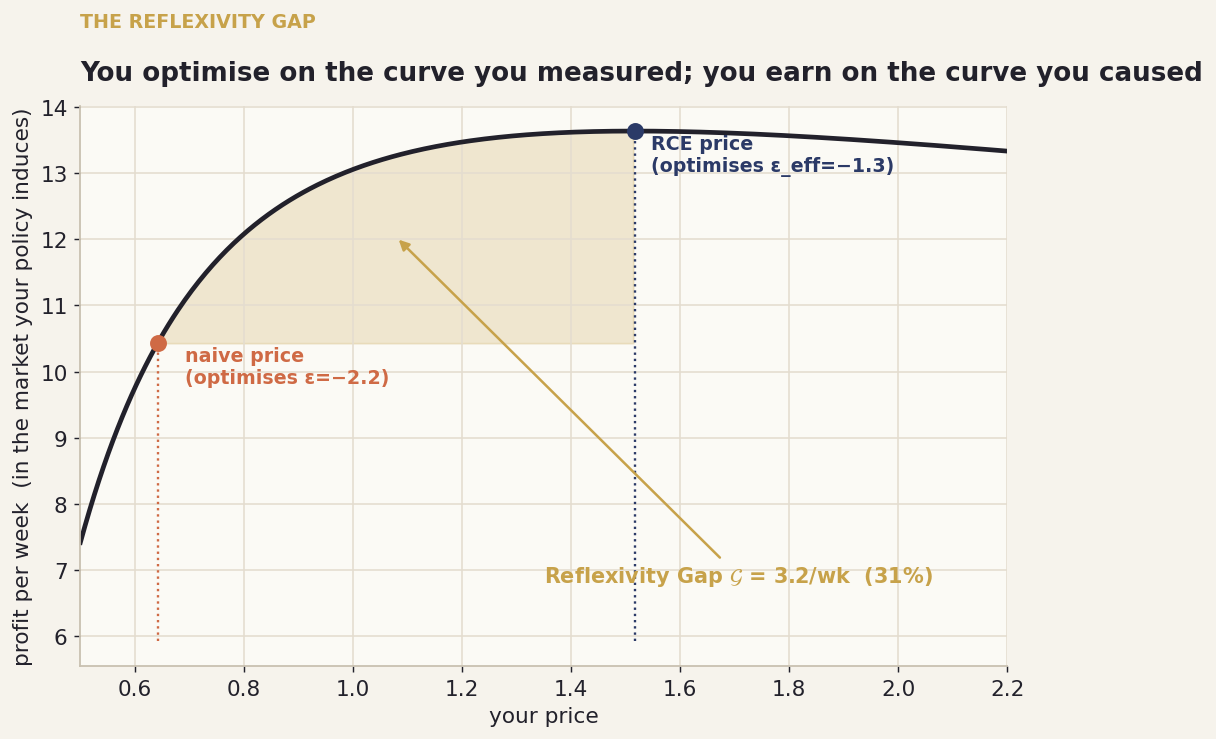
\includegraphics[width=.82\linewidth]{../figures/fig2_gap.png}
\caption{\textbf{The Reflexivity Gap.} Profit in the market the firm's own policy induces
($\epseff=-1.3$). Optimizing the measured static elasticity ($\epsown=-2.2$) places the firm at
the lower-left point; the RCE price sits at the peak. The shaded wedge is $\Gcal$---here about
$31\%$ of per-period profit, growing with competitor aggression (Proposition~\ref{prop:gap}).}
\label{fig:gap}
\end{figure}

\section{The reflexivity spectral radius}\label{sec:spectral}
Whether iterating $\Tcal$ (as any repeatedly re-estimating firm effectively does) converges is
governed by the modulus of its linearization.
\begin{definition}[Reflexivity spectral radius]
\[
\rhoR \;=\; \Big|\tfrac{d\,\mathrm{BR}}{da}\Big|\cdot\Big|\tfrac{da^*}{d\theta}\Big|\cdot\Big|\tfrac{d\hat\theta}{da}\Big|.
\]
\end{definition}
The three factors are, respectively, how strongly the competitor reacts, how strongly the firm's
optimal price moves with its belief, and how strongly the (imperfect) estimator's output moves
with the deployed price. When $\hat\theta$ is the two-sided estimator, the third factor is
(asymptotically) zero and $\rhoR=0$: Proposition~\ref{prop:rce}'s one-step convergence. The
diagnostic bites when the online estimator conflates the competitor's move with own-price
variation.

\paragraph{Closed form (linear instance).} Consider linear demand and linear reaction functions,
$q=\alpha+b_{\mathrm{own}}a+b_{\mathrm{cross}}c$ with $b_{\mathrm{own}}<0$, firm best response
$a^*(c)=(\alpha+b_{\mathrm{cross}}c-b_{\mathrm{own}}\mathrm{mc})/(-2b_{\mathrm{own}})$, and rival
reaction $c^*(a)=c_0+\kappa a$. The naive ``re-optimize each period against last observed price''
loop is the cobweb $a_{k+1}=a^*(c^*(a_k))$ with slope
\begin{equation}
\rhoR \;=\; \frac{\kappa\,b_{\mathrm{cross}}}{2\,|b_{\mathrm{own}}|}.
\label{eq:rho-linear}
\end{equation}
\begin{proposition}[Convergence dichotomy]\label{prop:dichotomy}
The cobweb has a unique fixed point $a^\star$ (the RCE) whenever $\rhoR\neq 1$. If $\rhoR<1$ the
iteration converges to $a^\star$ geometrically from any start; if $\rhoR>1$ it diverges for any
start $a_0\neq a^\star$.
\end{proposition}
\begin{proof}
The map is affine, $a_{k+1}=\rhoR\,a_k + \beta$ for a constant $\beta$ obtained by composing the
two affine responses, using $da^*/dc=b_{\mathrm{cross}}/(-2b_{\mathrm{own}})$ and $dc^*/da=\kappa$.
An affine map with slope $\rhoR$ has fixed point $a^\star=\beta/(1-\rhoR)$ for $\rhoR\neq1$ and
$|a_k-a^\star|=\rhoR^{\,k}|a_0-a^\star|$, which converges iff $\rhoR<1$ and diverges iff
$\rhoR>1$.
\end{proof}
Equation~\eqref{eq:rho-linear} yields the operational rule (illustrated in
Figure~\ref{fig:cobweb}): below the $\rhoR=1$ frontier, ship
and keep re-estimating; above it, a point estimate is a liability and the firm should hedge (Figure~\ref{fig:stability}).

\begin{figure}[t]
\centering
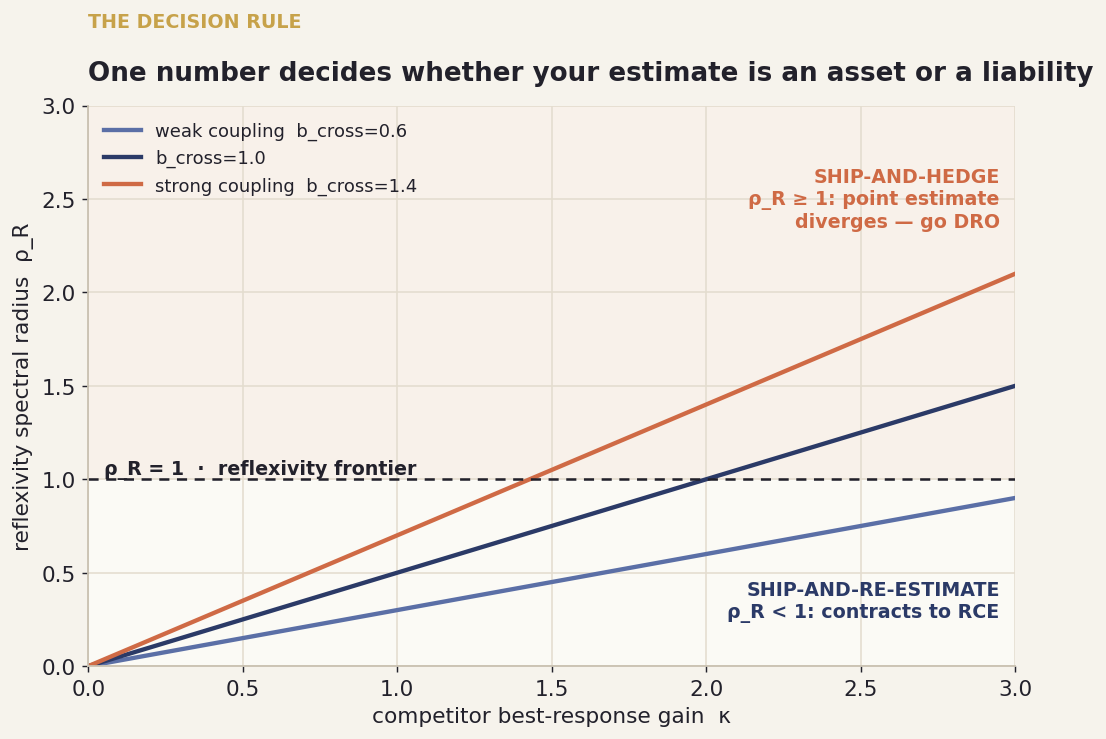
\includegraphics[width=.82\linewidth]{../figures/fig5_stability.png}
\caption{\textbf{The stability frontier.} As the competitor's response gain $\kappa$ and the
strength of cross-price coupling rise, $\rhoR$ climbs and crosses one. Below the frontier a point
estimate is an asset the agent should keep refreshing; above it, the same estimate diverges under
iteration and the agent switches to distributionally-robust pricing.}
\label{fig:stability}
\end{figure}

\section{The SHARP controller}\label{sec:controller}
SHARP operationalizes \S\ref{sec:operator}--\ref{sec:spectral} as a per-period loop.
\begin{enumerate}
\item \textbf{Sense.} On a trailing window, run two-sided IV--DML for $(\epsown,\epscross)$ and fit
the competitor best-response gain $\kappa$ and latency.
\item \textbf{Detect.} Monitor CUSUM of the structural-model residuals and the first-stage $F$
statistic. A CUSUM alarm signals a regime change; $F$ below a floor signals that the instrument
is no longer alive.
\item \textbf{Reason.} Form the reflexivity proxy
$\hat\rho = |\kappa|\cdot|\epscross/(1+\epsown)|$, a scale-appropriate estimate of the loop gain.
\item \textbf{Act.} If the instrument is dead, price by DRO over an ambiguity set of
$(\kappa,\epscross)$; else if a regime change is detected or $\hat\rho\ge\rho^*$, price the
Stackelberg objective with $c=\mathrm{BR}(a)$ folded in; else price the snapshot optimum.
\end{enumerate}
In the static regime SHARP reduces to the snapshot agent (as it should, by
Proposition~\ref{prop:rce}); it changes objective only when evidence warrants (Figure~\ref{fig:regime}).

\begin{figure}[t]
\centering
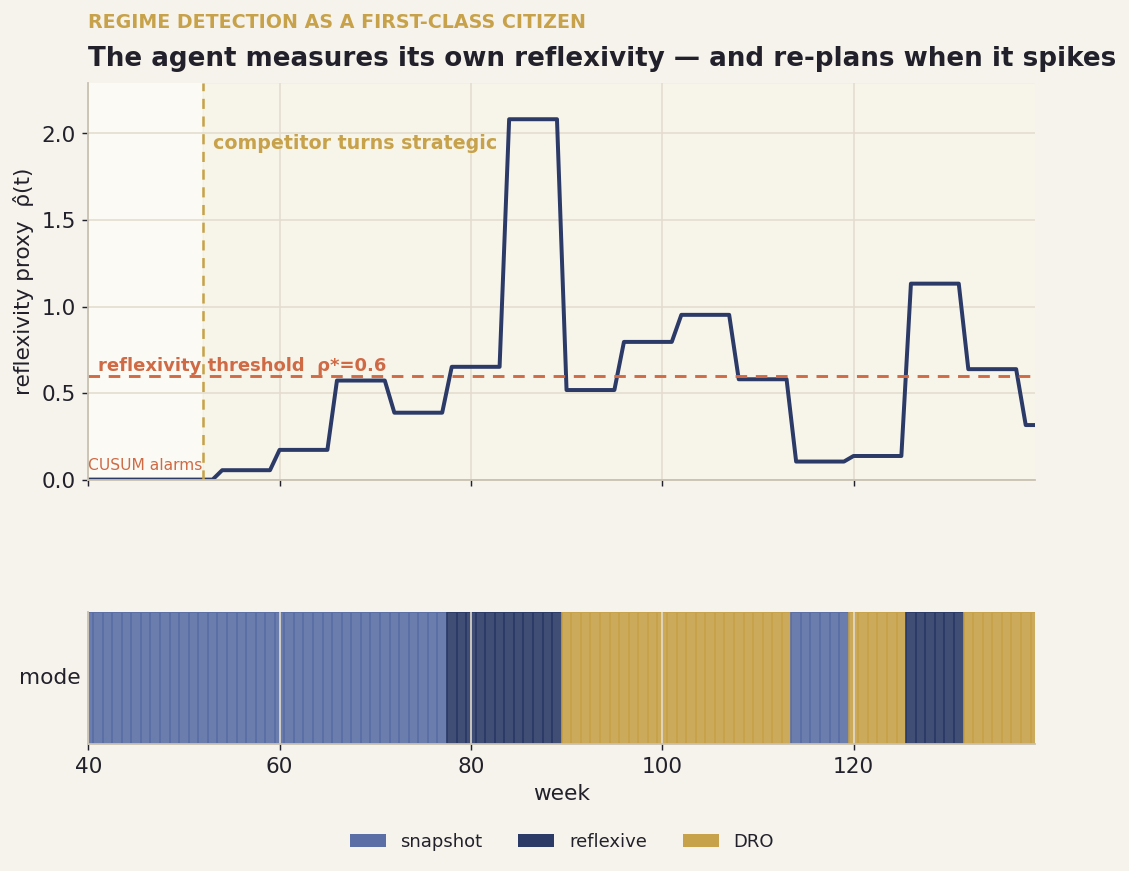
\includegraphics[width=.82\linewidth]{../figures/fig4_regime.png}
\caption{\textbf{The agent sensing its own reflexivity.} Before the break, the reflexivity proxy
$\hat\rho\approx0$ and SHARP stays in snapshot mode. When the competitor turns strategic,
$\hat\rho$ spikes past the threshold and CUSUM alarms fire; the mode timeline (bottom) flips into
reflexive (Stackelberg) and hedged (DRO) pricing.}
\label{fig:regime}
\end{figure}

\section{Experiments}\label{sec:experiments}
\paragraph{Setup.} We simulate the reflexive market with a discrete-event engine (weekly clock;
scheduled regime break, best-response arrivals with latency, estimate-expiry events). Structural
truth: $\alpha=3.0$, $\epsown=-2.2$, $\epscross=1.0$, $\kappa=0.9$, $L=3$, $\mathrm{mc}=0.35$,
giving $\epseff=-1.3$. Both agents warm up for 40 weeks; the competitor turns strategic at week
52; horizon 140 weeks. The baseline (\emph{Naive snapshot}) ships one correct single-IV estimate
of the static elasticity and prices against a frozen competitor thereafter---optimal in the
static regime, so the comparison is not against a strawman. We report cumulative profit from the
end of warmup over 12 seeds.

\paragraph{Identification.} The online single-IV baseline recovers $\hat\epsown=-2.31\pm0.33$
(true $-2.20$) with first-stage $F=415\pm141$: clean identification, so the trap that follows is
a decision failure, not an estimation failure.

\paragraph{Main result.} Table~\ref{tab:main} summarizes. SHARP wins $11/12$ seeds, pays a
statistically negligible premium pre-break ($-0.3\%$), and gains $+17.2\%$ post-break
($+14.1\%$ overall; paired $t=6.7$, $p<10^{-4}$). Figure~\ref{fig:trap} shows the mechanism: the
agents are indistinguishable until the break, after which the naive price stays pinned at the
static optimum while SHARP climbs toward the equilibrium optimum.

\begin{table}[t]
\centering
\begin{tabular}{lccc}
\toprule
Metric & Naive snapshot & SHARP & Difference \\
\midrule
Seeds won (of 12) & 1 & \textbf{11} & --- \\
Cumulative profit (post-warmup) & $1708\pm222$ & $\mathbf{1941\pm223}$ & $+14.1\%$ \\
Uplift, pre-break & --- & $-0.3\%$ & no premium \\
Uplift, post-break & --- & $\mathbf{+17.2\%}$ & where it counts \\
\bottomrule
\end{tabular}
\caption{Head-to-head over 12 seeds. Paired $t$-test on post-warmup profit: $t=6.7$, $p<10^{-4}$.}
\label{tab:main}
\end{table}

\begin{figure}[t]
\centering
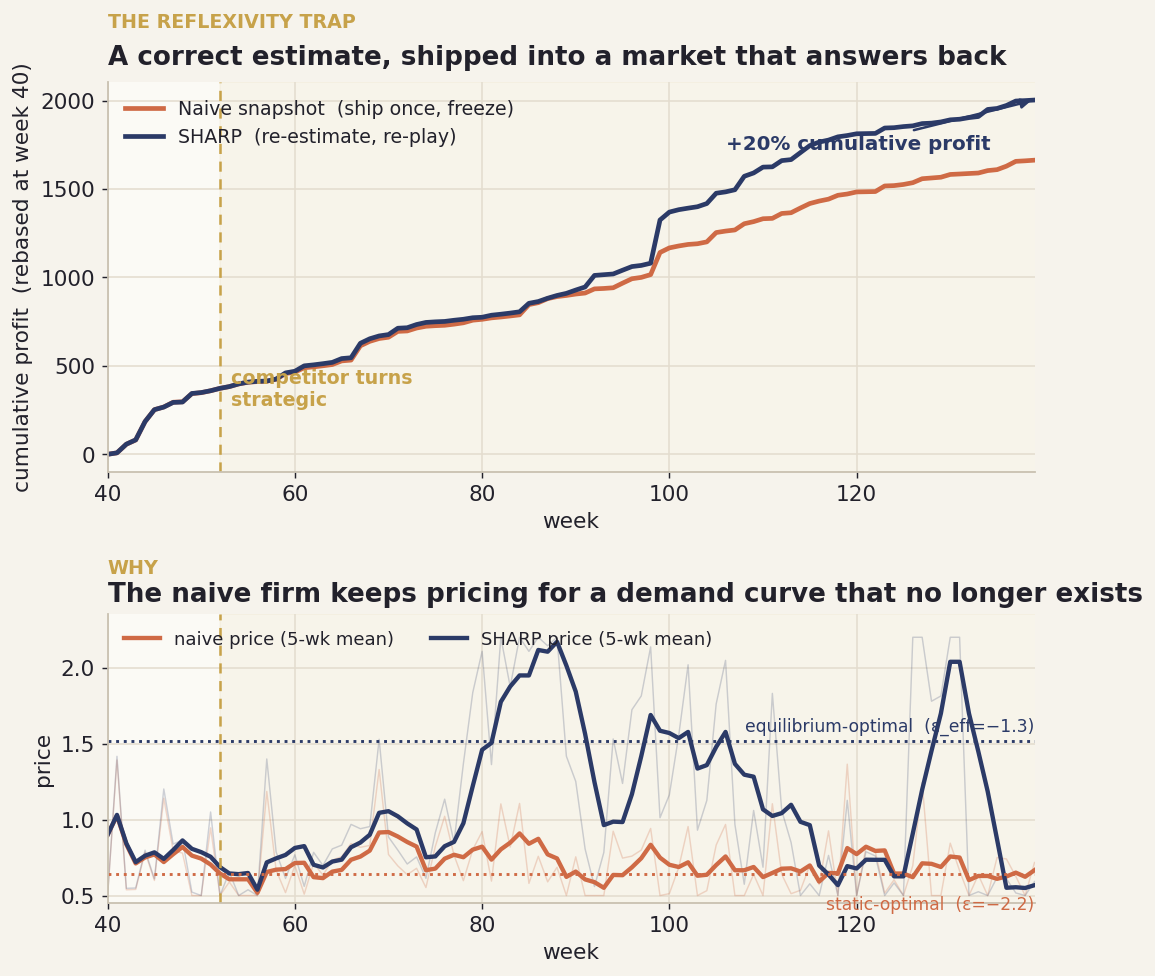
\includegraphics[width=\linewidth]{../figures/fig1_trap.png}
\caption{\textbf{The reflexivity trap.} Top: cumulative profit; the paths separate only after the
competitor turns strategic. Bottom: the naive firm holds the static-optimal price while SHARP
moves toward the equilibrium-optimal price.}
\label{fig:trap}
\end{figure}

\begin{figure}[t]
\centering
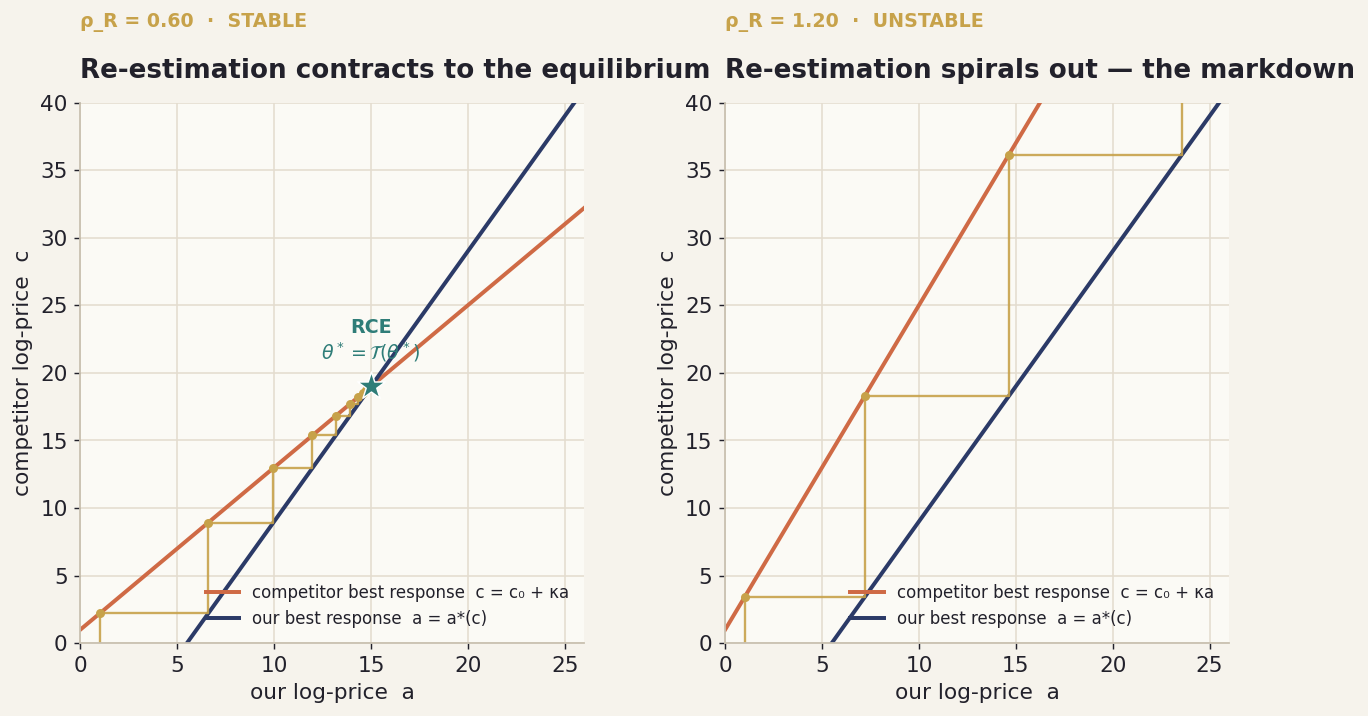
\includegraphics[width=.86\linewidth]{../figures/fig3_cobweb.png}
\caption{\textbf{Operator dynamics (linear instance).} $\rhoR<1$ contracts to the RCE (left);
$\rhoR>1$ diverges (right), matching Proposition~\ref{prop:dichotomy}.}
\label{fig:cobweb}
\end{figure}

\paragraph{Portfolio.} Scoring a three-market book by mean profit penalized by the CVaR of its
post-break drawdown, SHARP raises mean profit ($2246\to2932$), cuts the tail drawdown roughly
ninefold ($1329\to147$), and triples the risk-adjusted score ($918\to2785$). It also reallocates
toward the most competitive market, which it can now defend---reflexivity management changes
portfolio construction, not just point decisions.

\section{Case study: reflexivity in pharmaceutical pricing}\label{sec:pharma}
The mechanism is not hypothetical. Two documented episodes in competitive therapeutic classes
show a price set as if the rival would hold still, then matched once deployed.

\emph{PCSK9 inhibitors (2018--19).} Amgen's Repatha and Sanofi/Regeneron's Praluent both launched
near \$14{,}000/year in 2015, priced against cost-effectiveness thresholds in isolation~\cite{pcsk9}; payers
largely rejected them and uptake stalled. In late 2018 Amgen cut Repatha's list price roughly
$60\%$ to \$5{,}850; months later Regeneron and Sanofi matched Praluent to the identical
\$5{,}850---a rare public tit-for-tat on pre-rebate list prices. The value-based price was correct
for a market with a passive rival and passive payers, and wrong for the one it helped create.

\emph{GLP-1 agonists (2025--26).} In the obesity/diabetes duopoly of Novo Nordisk
(Wegovy/Ozempic) and Eli Lilly (Zepbound/Mounjaro), Novo cut cash prices from \$499 to \$349 per
month; within weeks Lilly best-responded with further cuts on its direct-to-consumer channel, and
Novo subsequently slashed list prices $35$--$50\%$. Cross-brand share moved materially over the
same window. The response latency is measured in weeks, faster than most re-estimation cadences~\cite{glp1}.

\paragraph{Why this is a sharper instance, not a weaker one.} Pharma adds structure that makes the
reflexive framing \emph{more} apt, not less. (i) The decision surface is the \emph{net} price and
formulary access, rebate-mediated through pharmacy benefit managers; list-price moves are often
around the pre-existing net price, so na\"ive list-price elasticity is doubly misleading. (ii)
Exogenous \emph{policy} regime shifts (the Inflation Reduction Act's Medicare negotiation;
government direct-purchase deals) coincide with competitive activation---precisely the
regime-change signal SHARP's detector is built to catch. (iii) Payer/rebate uncertainty is a
natural ambiguity set for the distributionally-robust mode. The SHARP objects map directly:
two-sided instruments become own- and rival-net-price shifters (manufacturing cost, exogenous
policy timing); regime detection fires on rival activation or a policy shock; DRO prices under
payer ambiguity when the instrument for net demand weakens.

\paragraph{Scope.} The framing applies to \emph{competitive branded} classes with two or more
rivals contesting access. It does \emph{not} apply during patent-protected monopoly, where there
is no strategic responder; there the ordinary (non-reflexive) causal estimate suffices.

\paragraph{Calibrated benchmark.} Re-instantiating the benchmark for a branded duopoly with
rebate-mediated net demand (net-revenue elasticity $\epsown=-1.7$, cross $\epscross=0.9$, rival
gain $\kappa=1.0$, short latency, low biologic COGS, with the regime break modelling combined
rival-plus-policy activation), SHARP wins $8/8$ seeds with a mean $+28\%$ cumulative net-revenue
uplift; by Proposition~\ref{prop:rce} it reduces to the snapshot agent before activation, so the
gain concentrates post-break (Figure~\ref{fig:pharma}). These parameters are an illustrative
calibration to the documented dynamics, not measured elasticities.

\begin{figure}[t]
\centering
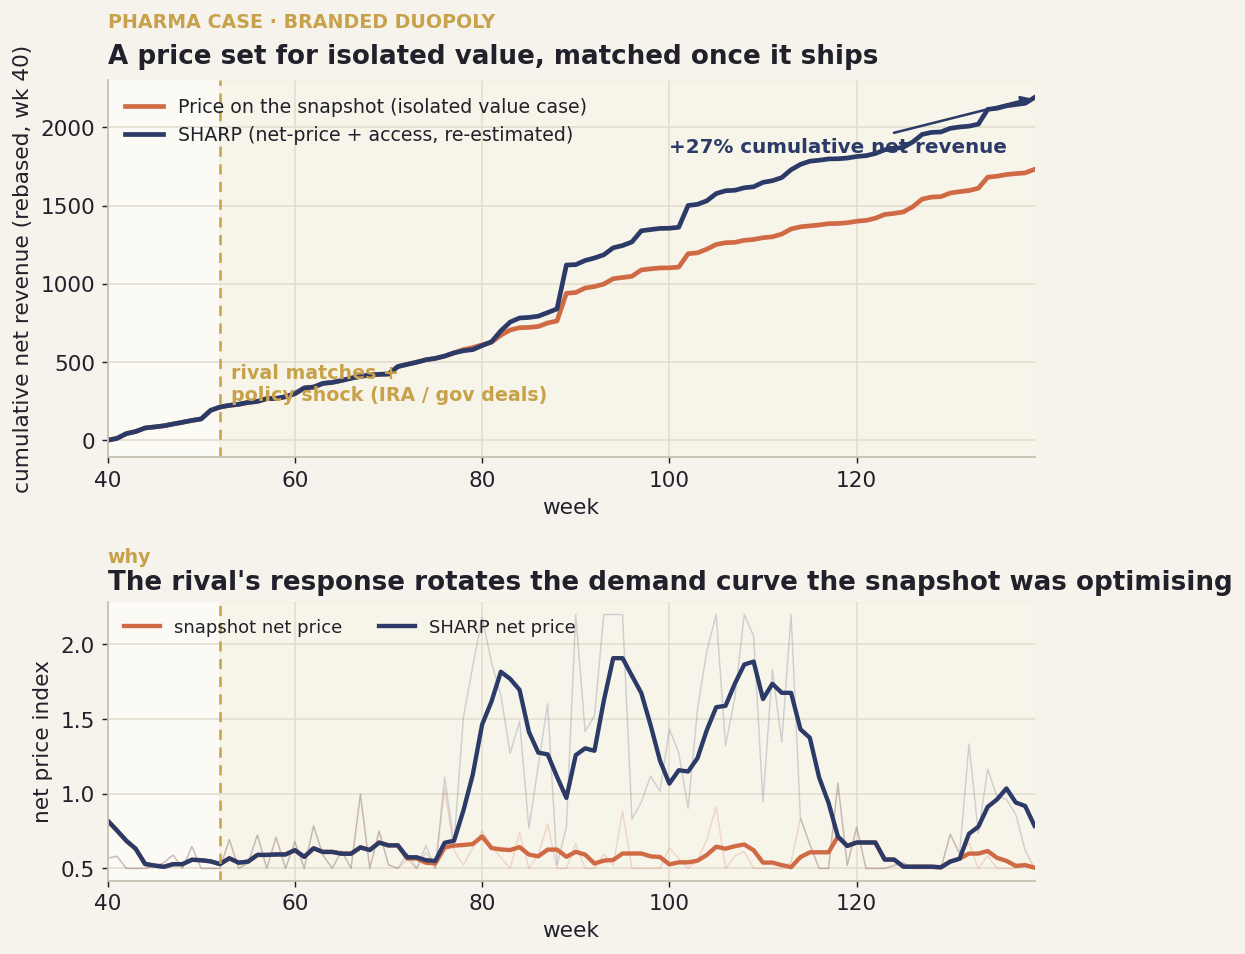
\includegraphics[width=.82\linewidth]{../figures/fig6_pharma.png}
\caption{\textbf{The reflexive trap in a branded therapeutic duopoly (calibrated).} A price set
for isolated value is matched once deployed and, together with a coincident policy shock, the
demand curve rotates; SHARP re-estimates the net-price/access game and pulls ahead. Calibrated to
the qualitative GLP-1 and PCSK9 dynamics, not fitted to firm financials.}
\label{fig:pharma}
\end{figure}

\section{Limitations}
The competitor is a parametric best-response with a single gain and latency; real rivals are
messier and may themselves be learning, raising the open two-adaptive-agents problem. Demand is
constant-elasticity; richer forms change the optimizer but not the operator logic. $\rhoR$ is
estimated by finite differences and inherits their noise. The benchmark is a simulation---faithful
to the mechanism but not a market. The results should be read as evidence that the mechanism
behaves as the theory predicts.

\section{Conclusion}
Causal estimates in strategic markets are photographs of a world that agreed to hold still. When
the world looks back---as competitors do---the estimate that was correct becomes the estimate that
bleeds. SHARP reframes the task from producing a durable estimate to running an agent that knows
the expiry date of its own beliefs: it re-estimates while it can, hedges when it cannot, and
prices the game rather than the snapshot. The Reflexive Operator, the Reflexivity Gap, and the
reflexivity spectral radius give that agent a principled, estimable basis for those choices.

\begin{thebibliography}{9}
\bibitem{lucas1976} R.~E. Lucas. Econometric policy evaluation: A critique.
\emph{Carnegie-Rochester Conference Series on Public Policy}, 1976.
\bibitem{perdomo2020} J.~Perdomo, T.~Zrnic, C.~Mendler-D\"unner, M.~Hardt. Performative
prediction. \emph{ICML}, 2020.
\bibitem{narang2023} A.~Narang, E.~Faulkner, D.~Drusvyatskiy, M.~Fazel, L.~J.~Ratliff.
Multiplayer performative prediction: Learning in decision-dependent games. \emph{JMLR}
24(202), 2023.
\bibitem{piliouras2023} G.~Piliouras, F.-Y.~Yu. Multi-agent performative prediction: From global
stability and optimality to chaos. \emph{ACM EC}, 2023.
\bibitem{mandal2023} D.~Mandal, S.~Triantafyllou, G.~Radanovic. Performative reinforcement
learning. \emph{ICML}, 2023.
\bibitem{hardt2022} M.~Hardt, M.~Jagadeesan, C.~Mendler-D\"unner. Performative power.
\emph{NeurIPS}, 2022.
\bibitem{survey2025} Dissecting performative prediction: A comprehensive survey.
\emph{ACM Computing Surveys}, 2025.
\bibitem{chernozhukov2018} V.~Chernozhukov et al. Double/debiased machine learning for treatment
and structural parameters. \emph{The Econometrics Journal}, 2018.
\bibitem{delage2010} E.~Delage, Y.~Ye. Distributionally robust optimization under moment
uncertainty with application to data-driven problems. \emph{Operations Research}, 2010.
\bibitem{pcsk9} Fierce Pharma. PCSK9 price-cut matchup: Regeneron and Sanofi slash Praluent list
tag 60\%, matching Amgen's Repatha. 2019.
\bibitem{glp1} pharmaphorum. Novo Nordisk to cut GLP-1 prices in tough US market. 2026;
BioSpace, Novo slashes GLP-1 prices again. 2026.
\end{thebibliography}

\end{document}
